\chapter{RFX-Hunch: a closed example based on electron temperature}
\label{section:RFXhunch}

With the aim at selecting an informative example of plasma computation that the machine learning could be devoted to, we chose to look at the temperature profiles that are coming from the Soft X-Ray diagnostics at RFX. The particular choice had been mainly motivated by the fact that it provides an example that can be a good representative factor of the plasma global configuration, being at the same time not too complex to be handled by simple networks. The electron temperature profile represents indeed a very important clue for looking at the plasma state that is very often accessed by physicists during analysis: it can be seen as an instant property that is almost ergodic during the pulse, it is acquired with a good temporal resolution, and that can be related to the magnetic configuration for the chosen time sample.

A plasma is composed with a mixture of species characterized by their own mass and electric charge. As first approximation, the plasma may be considered as consisting of two fluids mixed together: the first composed by the electrons and the second by the ions, or to be more specific by all the other heavy species: ions, neutral atoms, and other compound molecules.

What matters for a fusion machine is actually the ions temperature because electrons are not directly involved on fusion process.
Nevertheless electrons acquire energy from the electric field, which energizes the plasma, and lose part of it through elastic or inelastic collisions; in this way the plasma can move energy from one fluid to the other. For this reason in \textit{Tokamaks} this represents a direct handle for plasma heating through \acs{ECRH} plants. In RFX we don't have such input and the electron temperature are almost directly related to the plasma current and the magnetic pressure (\textit{pinch} effect).
In addition the acquired profile represents a local information of the internal state of plasma giving a chance to see through the simple external configuration.

This holds for the Thomson scattering too, indeed: the SXR invese-transformed profile of the plasma bremsstrahlung radiation, and the intensity of the scattered light from TS, provide the same kind of measure being both of them related to electrons velocity.
However, as already discussed, the two diagnostics are not interchangeable as they present different characteristics. In particular the TS is known to provide a more accurate measure both in spatial resolution and in the accuracy of the acquired quantity; on the other hand the SXR measure even being quite noisy, easily biased by plasma-wall interaction debris of carbon and other materials, and usually presenting a set of reconstructed points that vary in position and in number, has a very fine grained resolution in the time domain.
In RFX we have the SXR3 time resolution of about $500 \mu s$



\section{Constructing the dataset} % SHAx

Once selected the set of signals that were thought to present all needed ingredient for reconstructing the plasma configuration a complete dataset able to comply with \Tensorflow input data of the fitting algorithms. Within the \acs{TF} framework a particular structure is devoted to represent such dataset; this structure is meant to provide a set of commodity routines that are used afterwards to handle the training process organization, such as: the split of training and validation data, the batching subdivision, the mapping for adapting to the particular model, applying data regularization algorithm (simple shuffling for example), and so forth.
For this reason making out fusion data compatible with this structure is a key point to have a flexible input for all possible constructed network and ML models. 
This structure is defined in a special \TF object class that can be simply included in python source directly reading a sequence array, a record array of structured data, or even a \Pandas \textit{dataframe}.

Although this is the actual structural output shape of our dataset we had to cope with the heterogeneity of our data sources: being part of the signal dataset coming from a \IDL data-structure array of a complex and accurate selection on relevant experiment pulses~\cite{Gobbin}, and part from raw or elaborated signals directly read from the global \MDSplus database of pulses.
For this reason we chose to make a first collection of all signal in a separate database that could be thought as a signal common cache of all the used components in the presented ML recipes.
This dataset represents also a further useful mean of data handling, being provided with tools such as: ordered or normalized subsets generator, or interactively selection of the missing data representative symbol (i.e. NaN flavors, zero float, negative sign, etc.).
Moreover an interactive collating signal selector has been implemented that can generate sets of arrays of signals data composed by sequence of inputs selected by name. In this way we could have a direct array of parameters by a simple query: for example with the string "\texttt{t\_Ip\_Vt\_Theta\_F}" the output would be a list of all times in all pulses made by arrays with [\textit{time}, \textit{plasma current}, \textit{toroidal loop voltage}, \textit{theta parameter}, \textit{reversal parameter}].

After the definition of the data the target \TF dataset adaptation has been done using the dedicated \TF \verb|Dataset.dataset_from_generator()| function. This is particularly useful because it can dynamically adapt to the particular input, and will be the suitable tool for the future enhancement to any possible dynamic source selection (i.e. the direct \MDSplus query or any other).
In the following a related code has been extrapolated from our dataset definition:
%
\begin{lstlisting}[language=Python, caption=Dataset from generator]
    def tf_tuple_compose(self, fields=[]):
        def clip(x):
            try: 
                if len(x) > self.dim: x=x[0:self.dim]
            except: pass
            return x
        def gen():
            import itertools
            for i in itertools.count(0):
                if i < len(self):
                    qsh = self[i]
                    yield tuple([ clip(qsh[n]) for n in fields])
                else:
                    return

        d0 = tuple([ clip(self[0][n]) for n in fields])
        types = tuple([tf.convert_to_tensor(x).dtype for x in d0])
        shape = tuple([np.shape(x) for x in d0])
        return tf.data.Dataset.from_generator(gen, types, shape)
\end{lstlisting}
%
here the generator function is the nested defined method called \verb|gen()| that yields the dataset components from a itertool object or simply return if we ran out of dataset bounds. The last is the defined identification of the sequence termination\footnote{this is not actually a mandatory behavior, we could have a function that generates new unseen data \textit{ad libitum} without haveing to cope with validation restrains or shuffling batches}.
Afterwards the extracted datum is packed in a \TF input tensor specifying tuples of its type and shape.

The final dataset was eventually composed by a list of arguments chosen from the list in~\Table{\ref{tab:database}}.
In particular concerning the electron temperature we composed the \textbf{te} elements as the y-axis and either \textbf{prel} or \textbf{rho} for the x-axis of the profile. 
\begin{table}[]
    \centering
    \begin{tabular}{l|l|l|l}
\textbf{tag} & \textbf{dtype} & \textbf{shape} & \textbf{description} \\
\hline
\verb|label      | & S10        & 1         &   pulse label with p\_number and time                 \\
\verb|pulse      | & np.int32   & 1         &   MDSplus pulse number                                \\
\verb|start      | & np.int32   & 1         &   start time                       \\
\verb|i_qsh      | & np.int32   & 1         &   number index of QSH in trend                        \\
\verb|tbordo     | & f4         & 1         &   temperature at the plasma border                    \\
\verb|tcentro    | & f4         & 1         &   temperature at plasma center                        \\
\verb|pos        | & f4         & 1         &   position of the maximum gradinet                    \\
\verb|grad       | & f4         & 1         &   estimated maximum gradient                          \\
\verb|n_ok       | & np.int32   & 1         &   number of valid temperature times in trend          \\
\verb|prel       | & f4         & (20,)     &   relative positions of the temperature profile       \\
\verb|rho        | & f4         & (20,)     &   remapped position of the temperature profile        \\
\verb|te         | & f4         & (20,)     &   acquired temperatures                               \\
\verb|Ip         | & f4         & 1         &   plasma current                                      \\
\verb|dens       | & f4         & 1         &   plasma density                                      \\
\verb|Te_dsxm    | & f4         & 1         &   temperature acquired by DSXM device                 \\
\verb|F          | & f4         & 1         &   reversal parameter                                  \\
\verb|TH         | & f4         & 1         &   theta striction parameter                           \\
\verb|POW        | & f4         & 1         &   Ohmic power released on plasma                      \\
\verb|VT         | & f4         & 1         &   loop toroidal voltage                               \\
\verb|VP         | & f4         & 1         &   loop poloidal voltage                               \\
\verb|B0         | & f4         & 1         &   root sum squared of the m=0 modes                   \\
\verb|B07        | & f4         & 1         &   amplitude of mode (0,-7)                            \\
\verb|B08        | & f4         & 1         &   amplitude of mode (1,-8)                            \\
\verb|B06        | & f4         & 1         &   amplitude of mode (1,-6)                            \\
\verb|B1         | & f4         & 1         &   root sum squared of the m=1 modes                   \\
\verb|B17        | & f4         & 1         &   amplitude of mode (0,-7)                            \\
\verb|B18        | & f4         & 1         &   amplitude of mode (0,-8)                            \\
\verb|B19        | & f4         & 1         &   amplitude of mode (0,-9)                            \\
\verb|NS         | & f4         & 1         &   dominant (1,-7) vs all the other m=1 modes          \\
\verb|mapro      | & f4         & (51,51)   &   reconstructed 2D map by SHEq code                   \\
\verb|xxg        | & f4         & (51,)     &   x-position grid for mapro                           \\
\verb|yyg        | & f4         & (51,)     &   y-position grid for mapro                           \\
\verb|n          | & i4         & (10,)     &   array of remapped modes                             \\
\verb|absBt_rm   | & f4         & (10,)     &   abs value for remapped $B_t$ at border              \\
\verb|argBt_rm   | & f4         & (10,)     &   arg value for remapped $B_t$ at border              \\
\verb|absBr_rm   | & f4         & (10,)     &   abs value for remapped $B_r$ at border              \\
\verb|argBr_rm   | & f4         & (10,)     &   arg value for remapped $B_r$ at border              \\
\verb|absFlux_rs | & f4         & (10,)     &   abs flux at resonance                               \\
\verb|argFlux_rs | & f4         & (10,)     &   arg flux at resonance                               \\
\verb|absBr_rs   | & f4         & (10,)     &   abs $B_r$ at resonance                              \\
\verb|argBr_rs   | & f4         & (10,)     &   arg $B_r$ at resonance                              \\
\verb|absBr_rp   | & f4         & (10,)     &   abs $B_r$ at plasma                                 \\
\verb|argBr_rp   | & f4         & (10,)     &   arg $B_r$ at plasma                                 \\
\verb|absBr_max  | & f4         & (10,)     &   abs $B_r$ maximum value                             \\
\verb|absFlux_max| & f4         & (10,)     &   abs flux maximum value
    \end{tabular}
    \caption{List of arguments for each element of the database where the input dataset is composed. }
    \label{tab:database}
\end{table}
From this point of view the generated signal can be seen just like the dummy example that has been used to investigate the properties of the variational autoencoder in section~\cref{section:VAE}; again we can see the variation on x-axis as an extension of the 1D signal to create a general function mapping in which the x-domain is the position on the direction of reconstructed measures and the y-domain is the related acquired temperature.
Beside the values of the actual y-axis temperature, the main difference from the previous generated dataset is that the related position, although being in the same way an ordered set, is not completely random, but the shift can be seen almost as an added structured noise.
This is in fact a slight simplification of the problem and for the model itself that relax the need of reconstructing the previously discussed \textit{elastic fit} factors in the latent space.
On the other hand what is reasonably to expect from those profile is a continuous passage from a flat low-temperature configuration to a central peaked curve where eventually the "\textit{hunch}" can be either centered or shifted depending on whether we are looking at a QSH or a MH configuration and also, in the former case, the actual poloidal position of the \textit{island} that directly depends on the phase of the running dominant mode.
It is nevertheless worth to be specified that both datasets, the dummy generated sum of gaussian envelops an the real temperature profiles, are formally identical in their public API. Therefore  any applied algorithm can be used with one or the other, with the same script structure; the main difference resides only in the supervised labelling: the real curves temperature profile does not provide the related associated label, that in the dummy case describes the generation class to which it belongs (previously named \textit{kind}).

%% FD-NT-27
\section{Handling missing data}

Within the input dataset, if any of \textbf{prel} or \textbf{rho} has been selected to describe the x-axis position on the electron temperature profile, it is almost immediate to see that the majority of samples is actually missing in some of the acquired position. This means that the number of real values for the corresponding line of sight have not been recorded. 
In the input dataset all arrays have been set to be left filled without spaces, from the minimum to the maximum x-position values, and a zero queue is left on the remaining. This is not acceptable to represent a valid network input as it would differently stimulate neurons with values that do not pertain to the same physical quantity, but are organized only by a favourable memory index.
A first reorganization was thus needed to define a set of new array position that are indexed on a the actual contained value basis.

The entire input array has been also defined over sized with respect to the complete acceptance of the actual positions. This means that the complete dataset could be reduced implementing a shrink of given set filling the gaps that have been left in these arrays. If all valid data - that account elements on the basis of a AND boolean operation between the non NULL data in x-position (either \textit{prel} or \textit{rho} arguments) and y-position (the Te temperature) - are reduced by sum along each element xy array, the overall distribution of the obtained sum values shows indeed a maximum of 18 counts, when the total size of each array is 20. Moreover, once the reordering of x-axis positions have been performed, and the zero populated elements removed, for some of the positions the NULL data persists again in almost the entire dataset (with very few exceptions). 

We finally decided to apply the reordering of the dataset x and y arrays using a k-means approach, defining the centroids on the basis of the x-value (i.e. the \textit{prel} position) on a total amount of $k=15$ clusters. This is actually a over constraint that loose some of the available information on the few input data that present more that 15 elements; however this allows to have a polluted set of positions to perform a useful training for all neurons that are facing the input features.
Another possible approach would have been to conversely apply a complete random position to the couple x-y leaving the network to perform a reordering on the firs layers; the casual selection on position is again needed to have a uniform population of input feature per neuron otherwise the training would expose an under-fitted set of weights on its internal kernel that would lead in turn to an undetermined local output on the network.
This refinement was not pursued at this first attempt though because we decided to maintain the overall needed network structure as simple as possible. In any event we leave it for a second stage of implementation to obtain a complete useful reconstruction of the profile.

That said, we are still facing a sparse input feature set where many values are NaN\footnote{NaN - litterally Not a Number - is a member of numeric data types to determine an undefined or unrepresentable value, especially in floating-point arithmetic. }. Unfortunately most generally available common implementations of neural network does not comply with NaN values. The common approach is to fill the empty gaps with a pre-computed value before the application to the neural network; this is commonly referred as \textit{data imputation} preconditioning. Many further approaches can be selected for this imputation algorithm, and a general accepted approach is a regression of some kind on the neighbour of missing data. This seemed a well documented and easy way to go at first glance; however in this dataset we are facing many adjacent missing data and a "simple" regression (polinomial or ridge) didn't produce a good fit for all the samples. 

Here comes the novel approach; as it has been already shown in~\cref{section:feedforward dense networks} we can see the network itself as a non linear regression operator, we could speculate that the network itself should be able to fill the gaps by means of available data, and it can also do this considering not only the single data under analysis, but the entire dataset.
Our very simple solution is sketched in~\Figure{\ref{fig:6_vae_missing}}
%
\begin{figure}
    \centering
    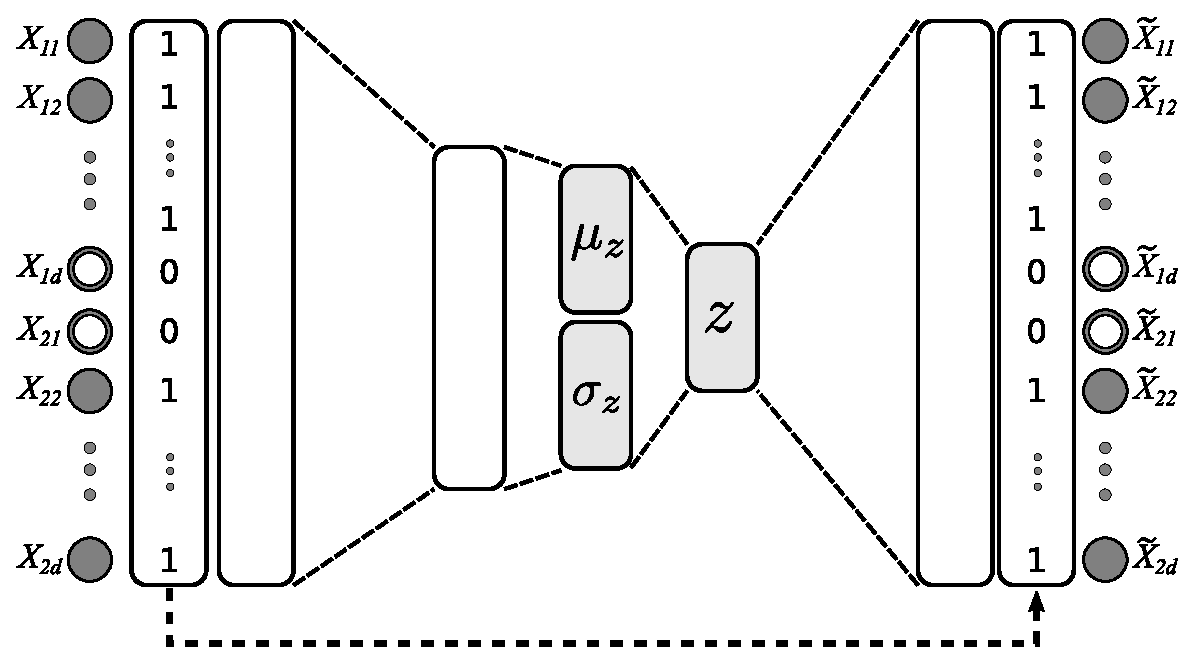
\includegraphics[height=6cm]{img/6_T_Hunch/VAE_MISSING.eps}
    \caption{VAE Missing point training NaN-Mask layer}
    \label{fig:6_vae_missing}
\end{figure}
%
where it can be seen that we applied the legacy \acs{VAE} schema with a sole couple of mirror layers added on the head and on the tail of the sample path through the network. In particular we added a simple input conditional layer, called \textbf{NaN-Mask} layer, that transforms all NaN to zero floats on the inference network, and at the same time the same mirrored transformation is applied on the network output erasing the generated network guess.
This is applied for all (and sole) training data; we chose to apply the zero float value to those inputs but any acceptable float would be equally accepted, because the magic is actually that the mirrored assignment on the output makes \textit{zero back-propagated error} for that input so the training simply does not see the missing data at all and proceed on training with the other available information.
\begin{figure}
    \centering
    \subfigure[]{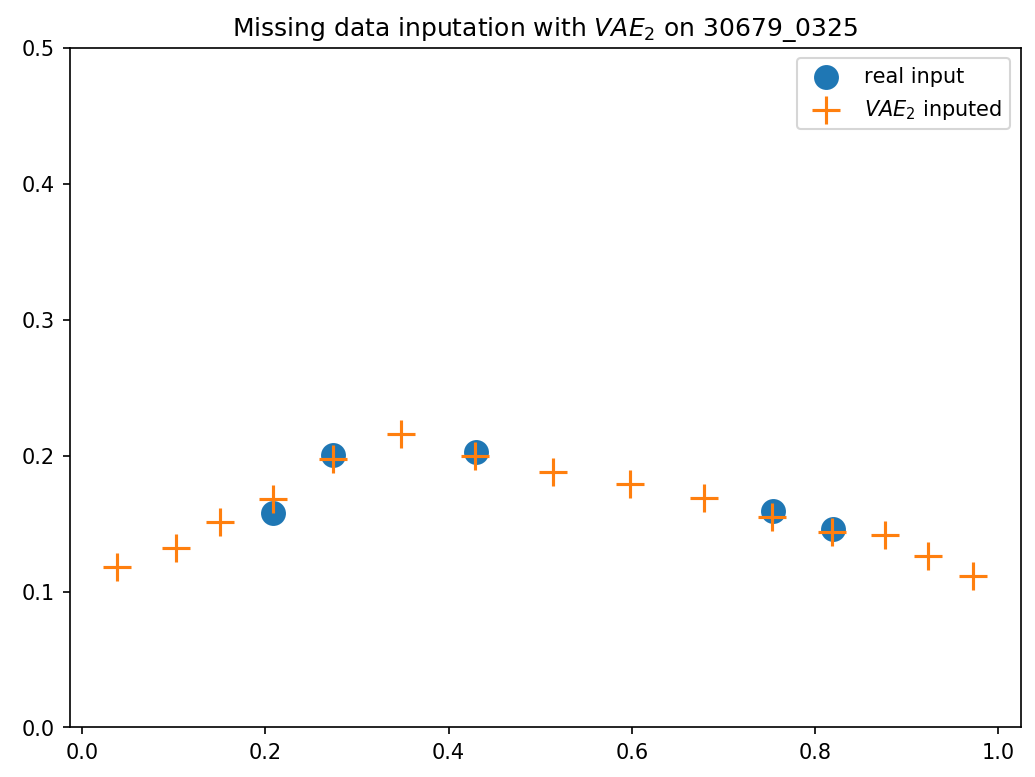
\includegraphics[width=5cm]{img/STEP7_CLEAN/missing_data_example.png}}
    \subfigure[]{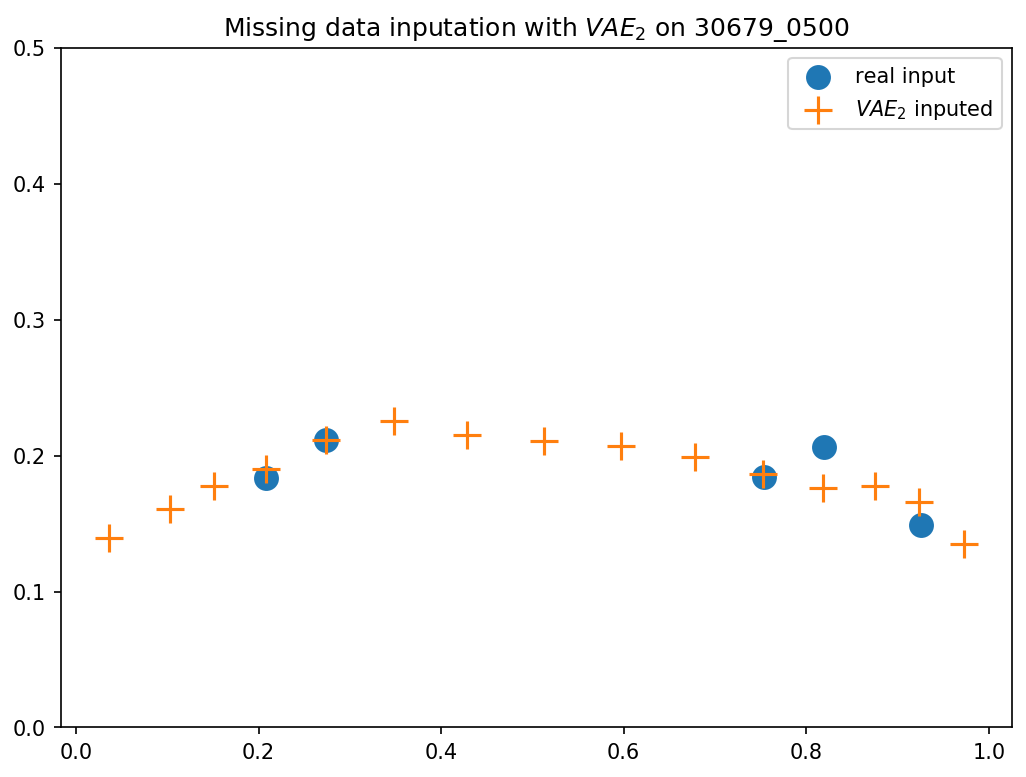
\includegraphics[width=5cm]{img/STEP7_CLEAN/missing_data_example2.png} label{fig:missing data example_b}}
    \caption{Missing data example as seen by a simple generated output of \VAE{2} trained with NaNMask layers, where only 5 valid element were present in the input profile (a)(b); a slight effect of VAE denoising is also visible in (b). }
    \label{fig:missing data example}
\end{figure}
Two examples of extreme missing data input have been proposed to a \VAE{2} model pre-trained with our NaN-Mask layers and are shown in~\Figure{\ref{fig:missing data example}}; on blue dots ($\bullet$) the input profile with missing points, and on red cross (+) the output of the network where the output mask layer is disabled guessing the profile form the reconstructed point in latent space.

\subsection{Data recovery and signal denoising}
In~\Figure{\ref{fig:missing data example}} an example of missing data recovery has been presented where a simple \VAE{2} model was able to generate the missing portion of the curve. The beauty of this imputing data approach, as already anticipated, is that the network proposes a regression that is based on available input data, but also on the complete dataset because it proposes an instance of a reconstructed space that comes form a likelihood maximized over the entire dataset.
However in~\Figure{\ref{fig:missing data example_b}} some points on the right side of the profile seem to be bad reconstructed, but this example was carefully selected to show on the contrary another concurrent effect of \acs{VAE} generative output: the data denoising.
This exploit the same principle that the reconstruction is treated scholastically, the effect is well known and fall into the category of \textbf{denoising autoencoders}.
Input aorrupting the data on purpose by randomly turning some of the input values to zero. In general, the percentage of input nodes which are being set to zero is about 50\%. Other sources suggest a lower count, such as 30\%. It depends on the amount of data and input nodes you have.
Usually a \textit{denoising autoencoder} is a overcomplete autoencoder that 


\begin{figure}
    \centering
    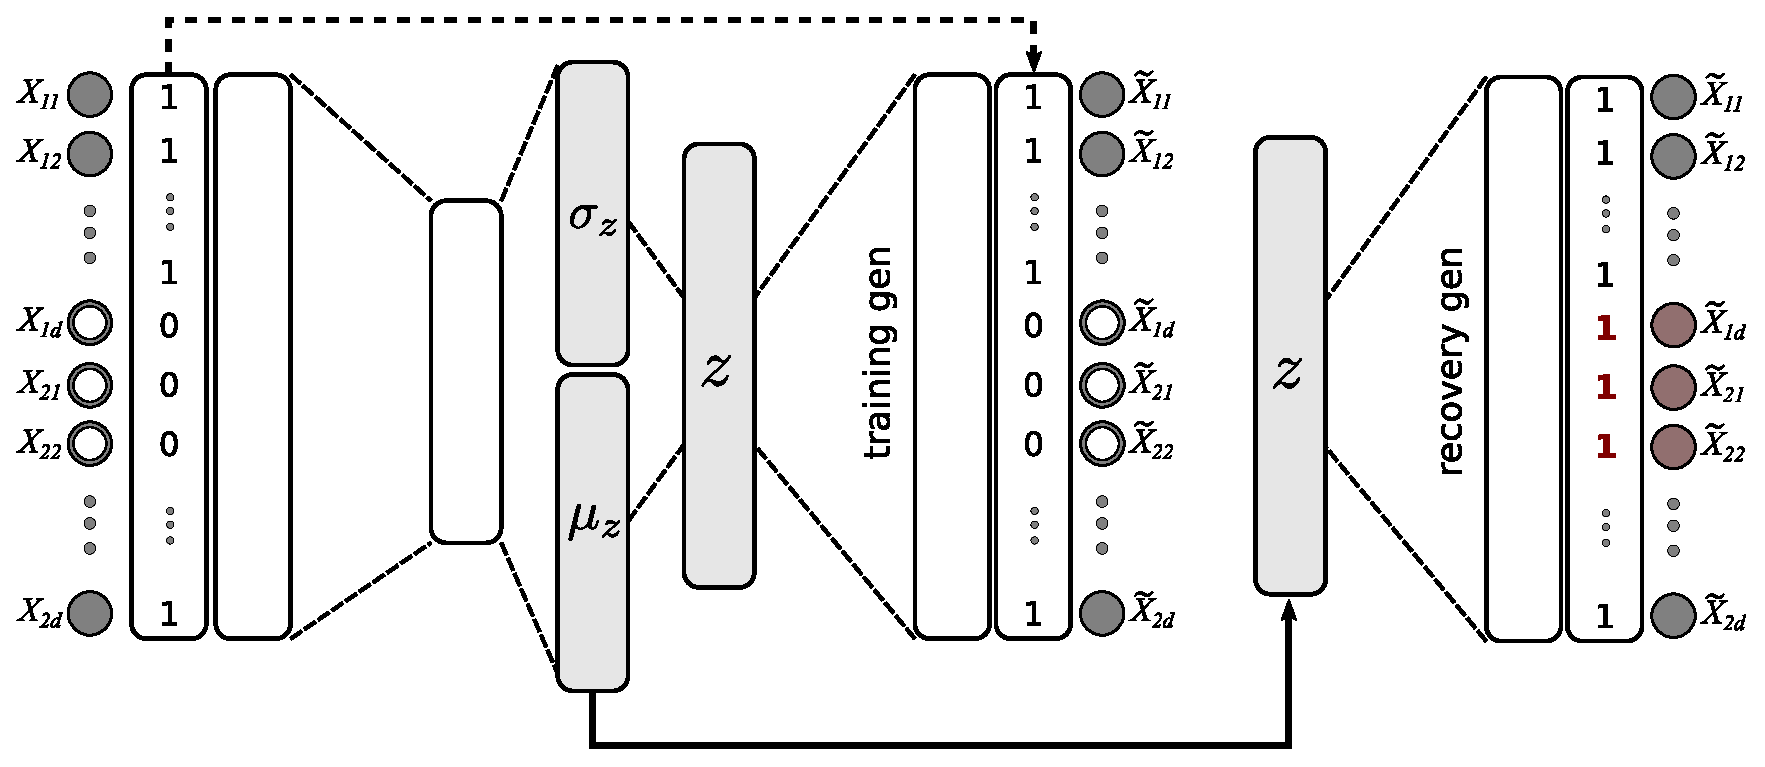
\includegraphics[height=6cm]{img/STEP7_CLEAN/VAE_CLEAN.eps}
    \caption{Recovery process of missing data}
    \label{fig:VAE_recovery}
\end{figure}



\begin{figure}
    \centering
    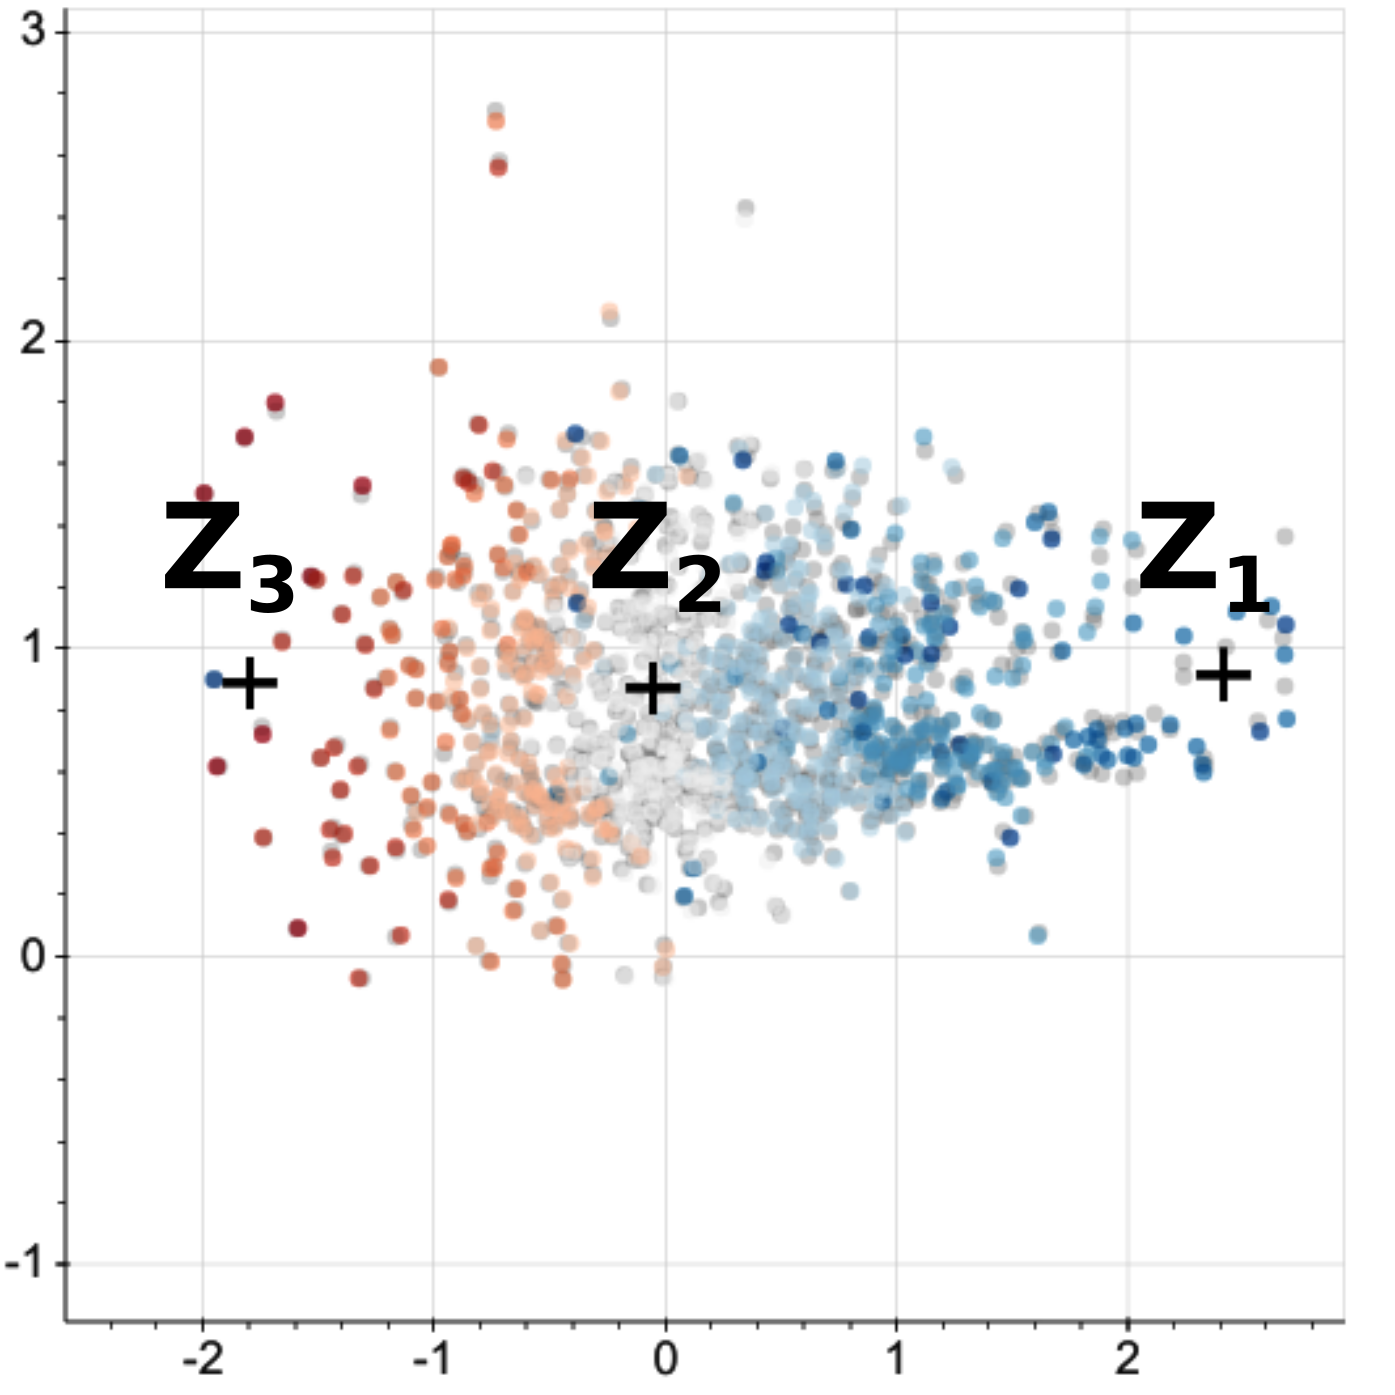
\includegraphics[height=6cm]{img/6_T_Hunch/ls_beta_tcentro_123.png}
    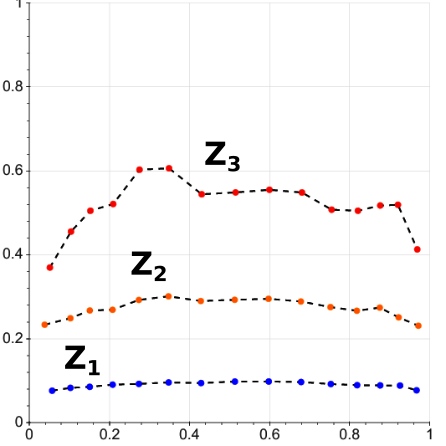
\includegraphics[height=6cm]{img/6_T_Hunch/ls_beta_tcentro_123_gen.png}
    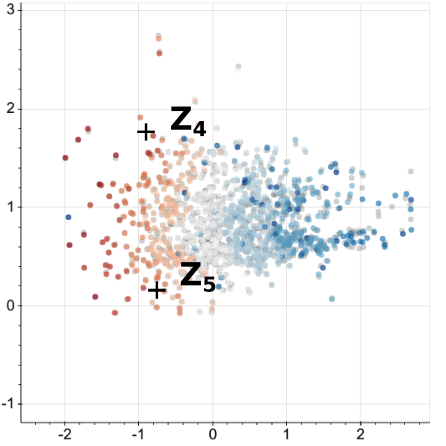
\includegraphics[height=6cm]{img/6_T_Hunch/ls_beta_tcentro_45.png}
    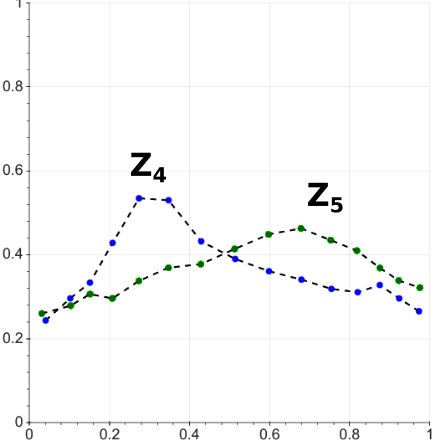
\includegraphics[height=6cm]{img/6_T_Hunch/ls_beta_tcentro_45_gen.png}
    \caption{VAE tcentro}
    \label{fig:my_label}
\end{figure}


\begin{figure}
    \centering
    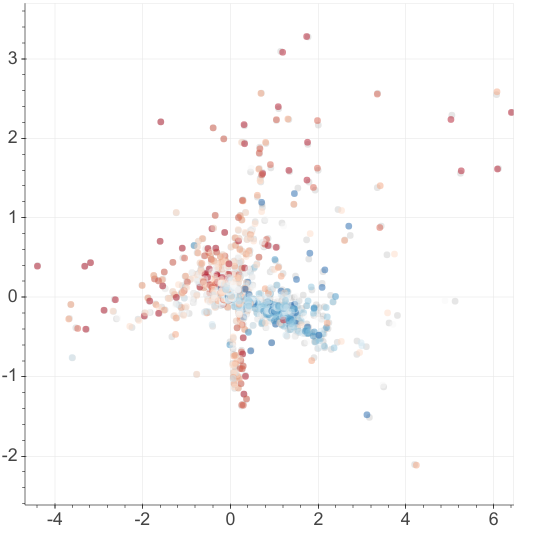
\includegraphics[height=6cm]{img/6_T_Hunch/ls_beta_clip_tcentro.png}
%    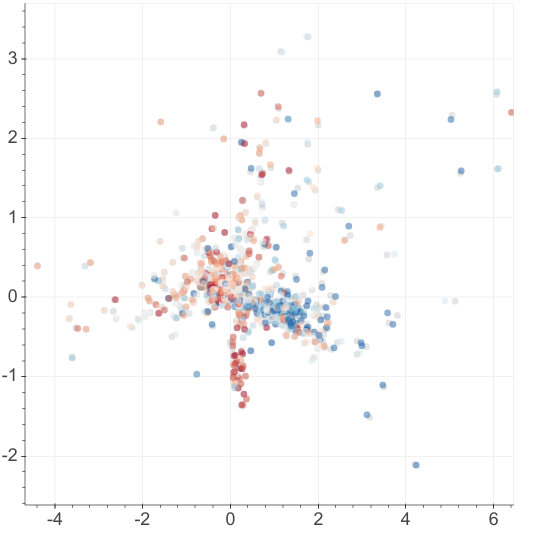
\includegraphics[height=6cm]{img/6_T_Hunch/ls_beta_clip_tbordo.png}
    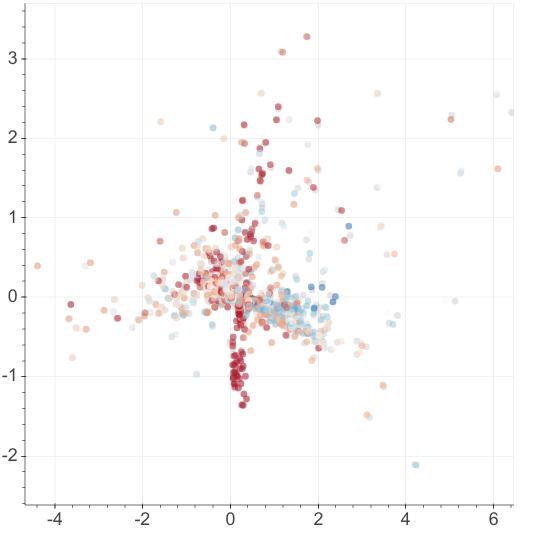
\includegraphics[height=6cm]{img/6_T_Hunch/ls_beta_clip_Ip.png}
    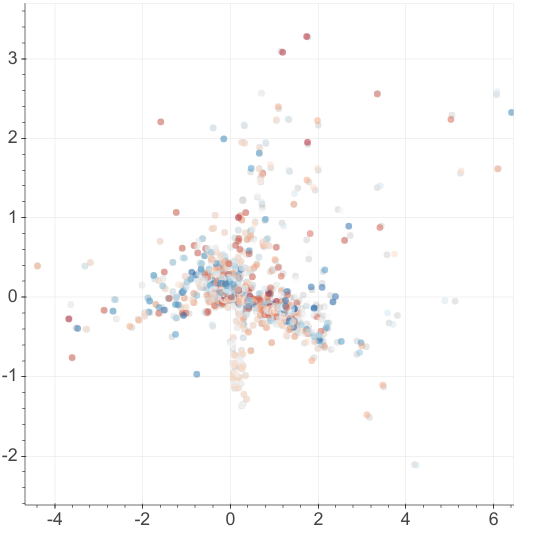
\includegraphics[height=6cm]{img/6_T_Hunch/ls_beta_clip_F.png}
    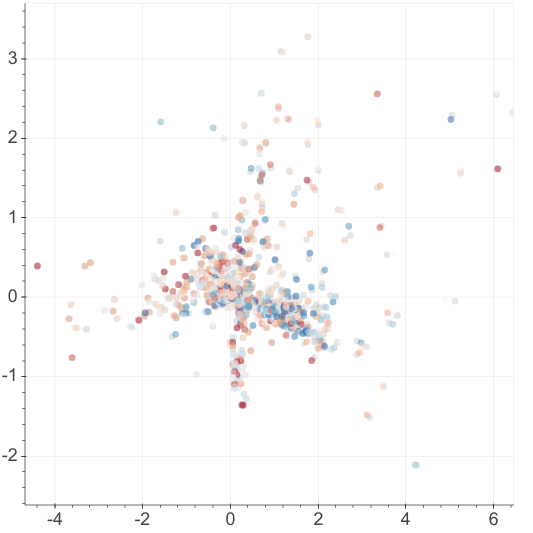
\includegraphics[height=6cm]{img/6_T_Hunch/ls_beta_clip_NS.png}
    \caption{VAE clip vs external info}
    \label{fig:my_label}
\end{figure}

\begin{figure}
    \centering
    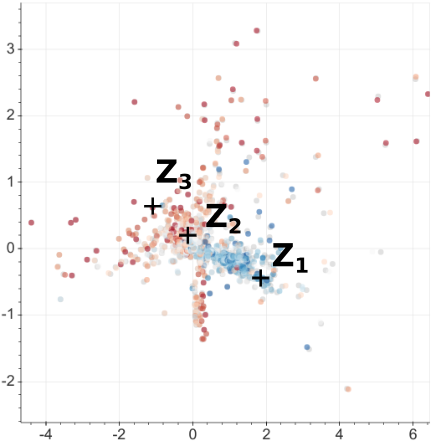
\includegraphics[height=6cm]{img/6_T_Hunch/ls_beta_clip_tcentro_123.png}
    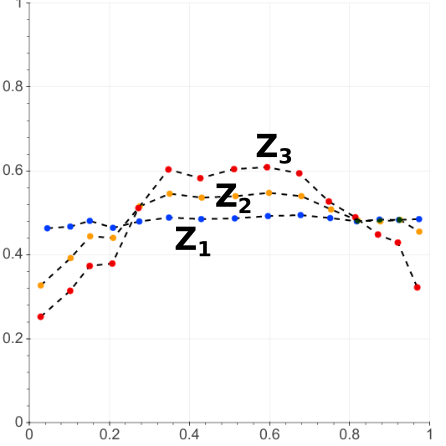
\includegraphics[height=6cm]{img/6_T_Hunch/ls_beta_clip_tcentro_123_g.png}
    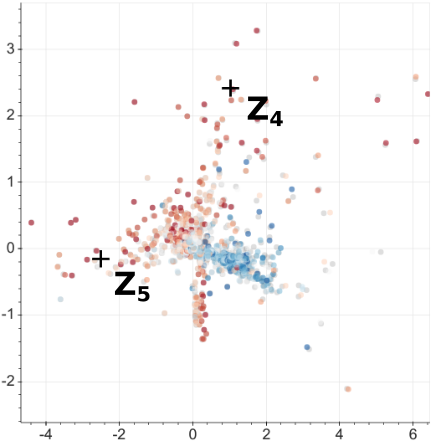
\includegraphics[height=6cm]{img/6_T_Hunch/ls_beta_clip_tcentro_45.png}
    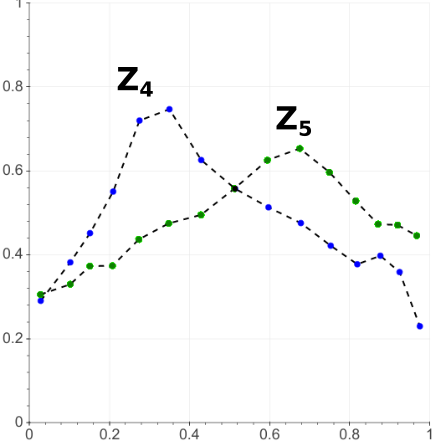
\includegraphics[height=6cm]{img/6_T_Hunch/ls_beta_clip_tcentro_45_g.png}
    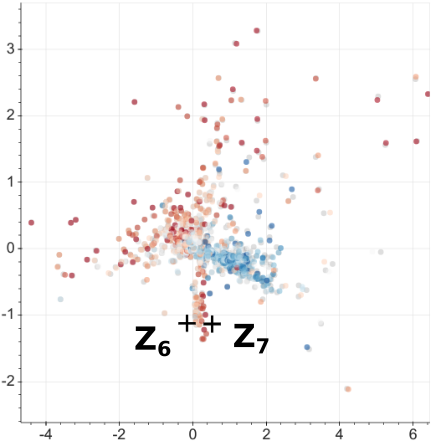
\includegraphics[height=6cm]{img/6_T_Hunch/ls_beta_clip_tcentro_67.png}
    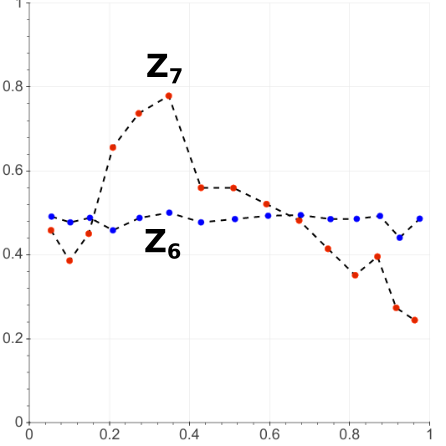
\includegraphics[height=6cm]{img/6_T_Hunch/ls_beta_clip_tcentro_67_g.png}
    \caption{VAE clip space}
    \label{fig:my_label}
\end{figure}

\section{( show using of dropout, rebalancing and beta )}


\section{composing VAEs}

\begin{figure}
    \centering
    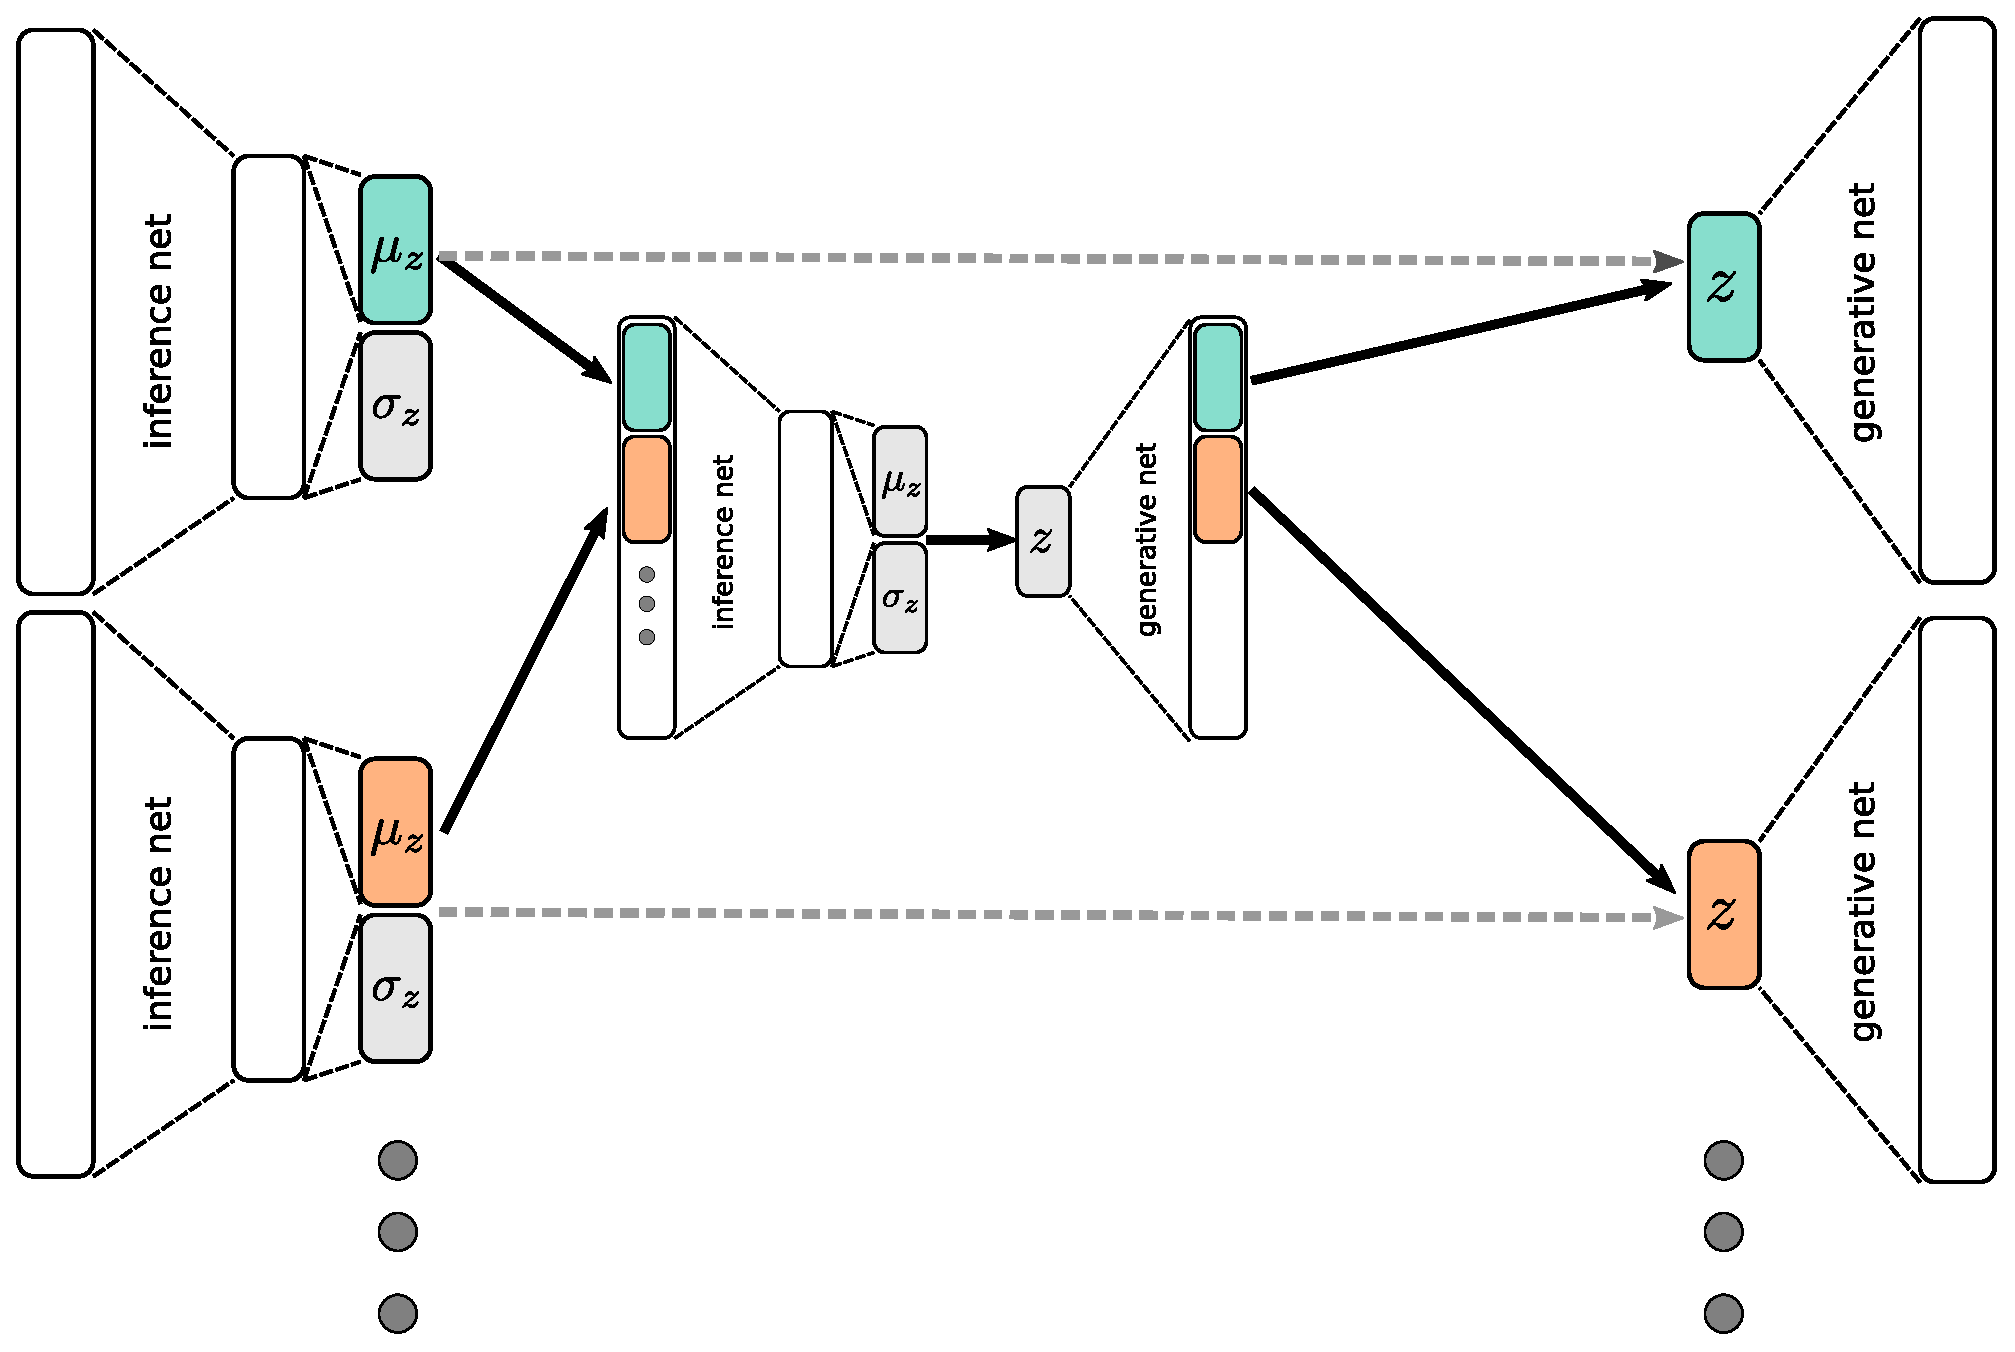
\includegraphics[height=6cm]{img/3_ML/VAE_COMPOSE.eps}
    \caption{Caption}
    \label{fig:my_label}
\end{figure}



\section{parameters to SXR mapping}



\section{Adding information through models ( Zanca-Terranova )}


\begin{figure}
    \centering
    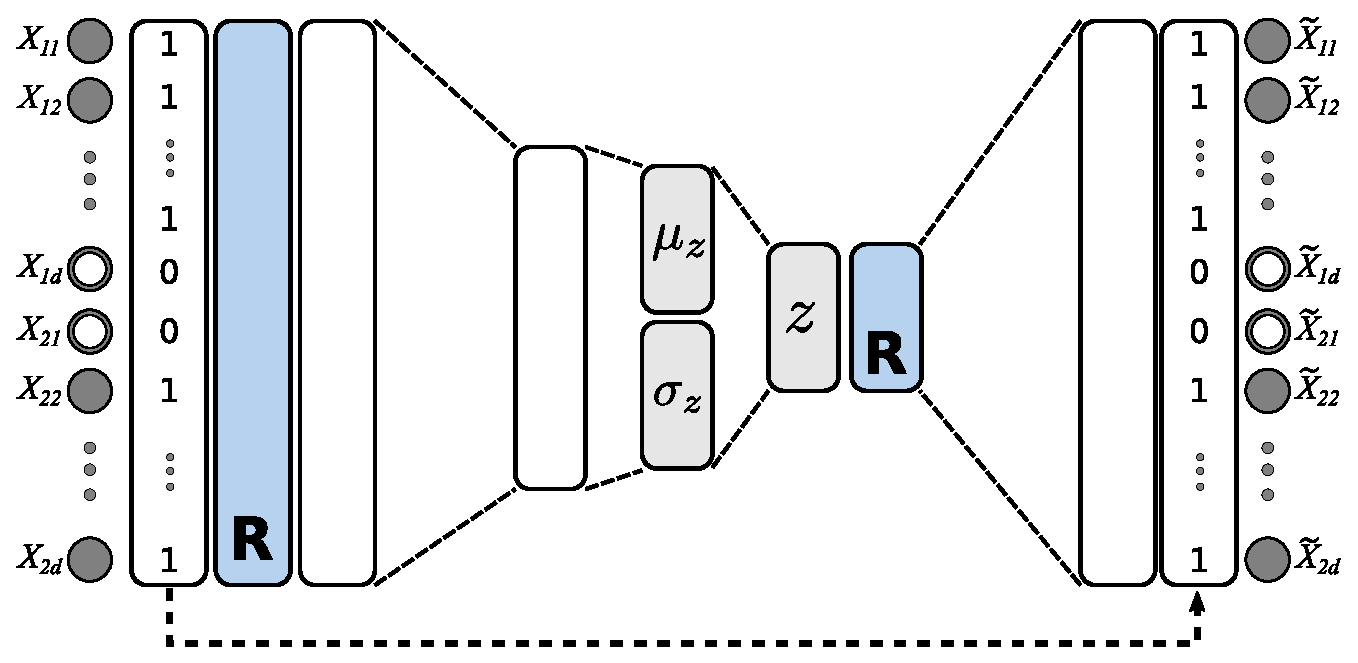
\includegraphics[height=6cm]{img/STEP12_7/VAE_RELEVANCE.eps}
    \caption{Relevance layer}
    \label{fig:my_label}
\end{figure}

\begin{figure}
    \centering
    \subfigure{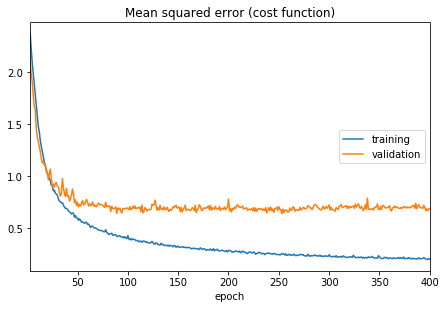
\includegraphics[height=3.3cm]{img/STEP12_7/STEP12_7_pBr2SXR_rm-rs_absarg_training_mse.png} \label{step_12_7_training}}
    \subfigure{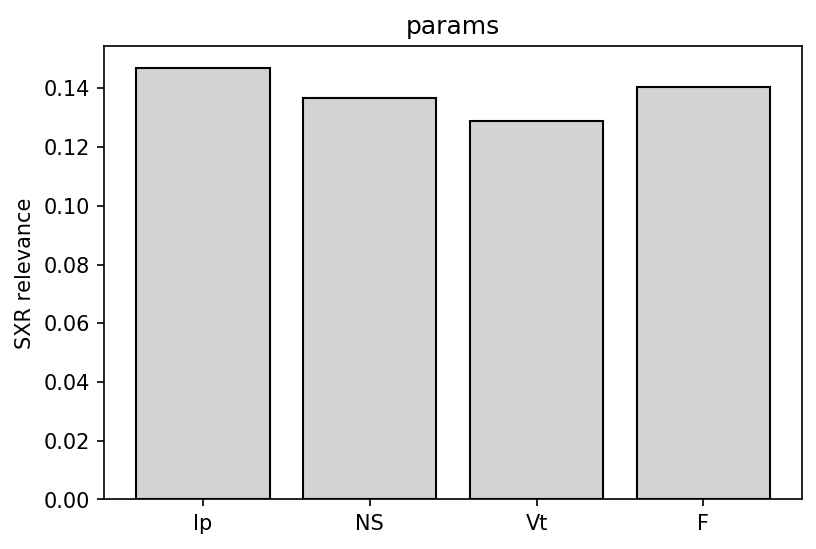
\includegraphics[height=3.3cm]{img/STEP12_7/STEP12_7_params.png} \label{step_12_7_p}}
    \subfigure{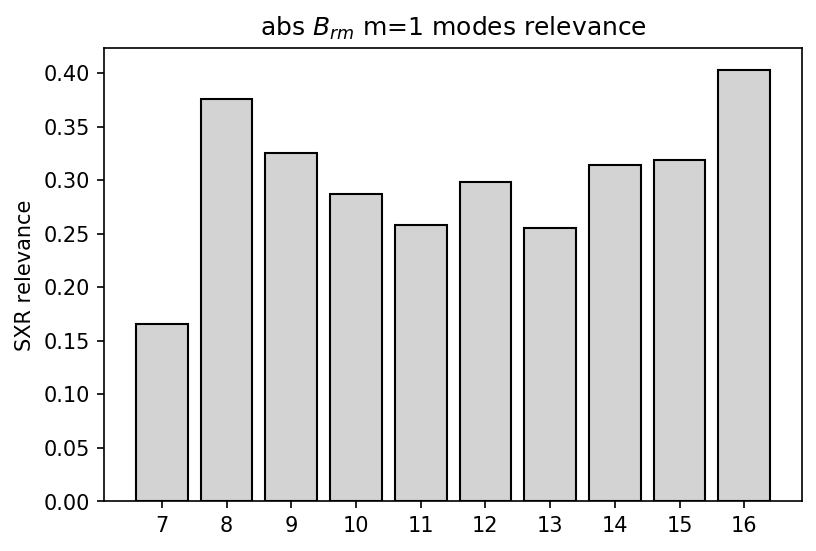
\includegraphics[height=3.3cm]{img/STEP12_7/STEP12_7_abs_Br_rm.png} \label{step_12_7_abs_Brm}}
    \subfigure{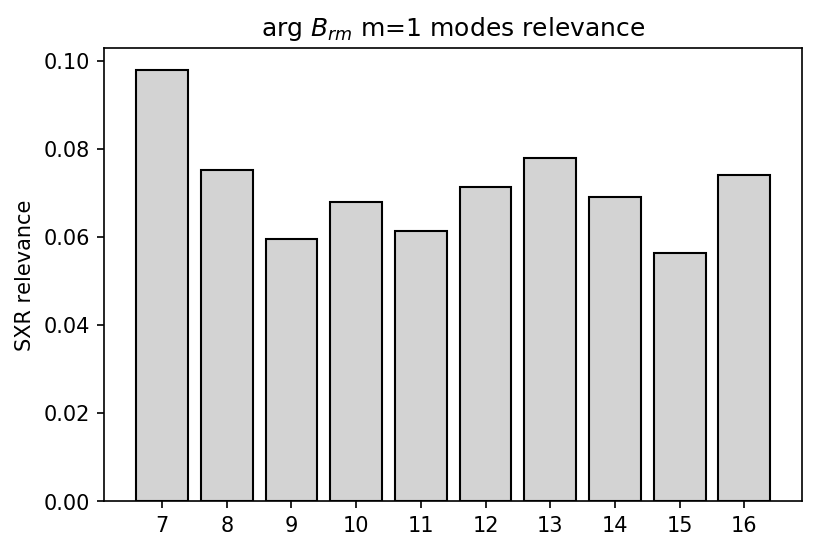
\includegraphics[height=3.3cm]{img/STEP12_7/STEP12_7_arg_Br_rm.png} \label{step_12_7_arg_Brm}}
    \subfigure{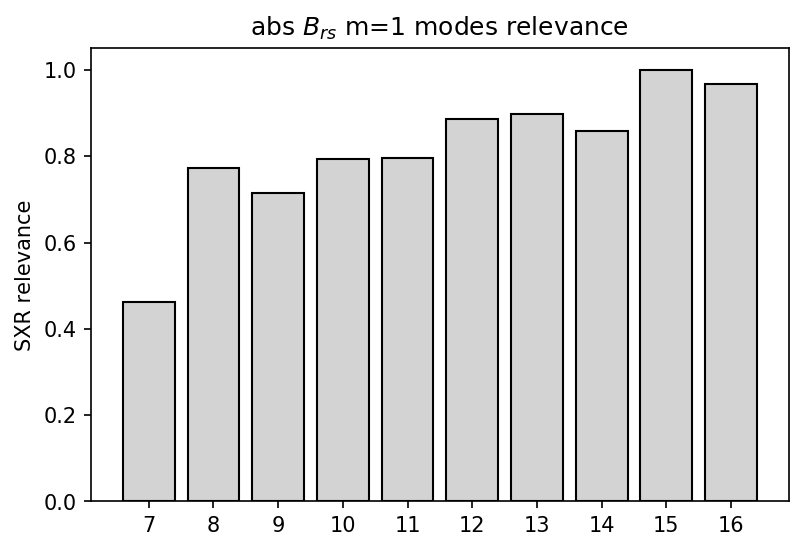
\includegraphics[height=3.3cm]{img/STEP12_7/STEP12_7_abs_Br_rs.png} \label{step_12_7_abs_Brs}}
    \subfigure{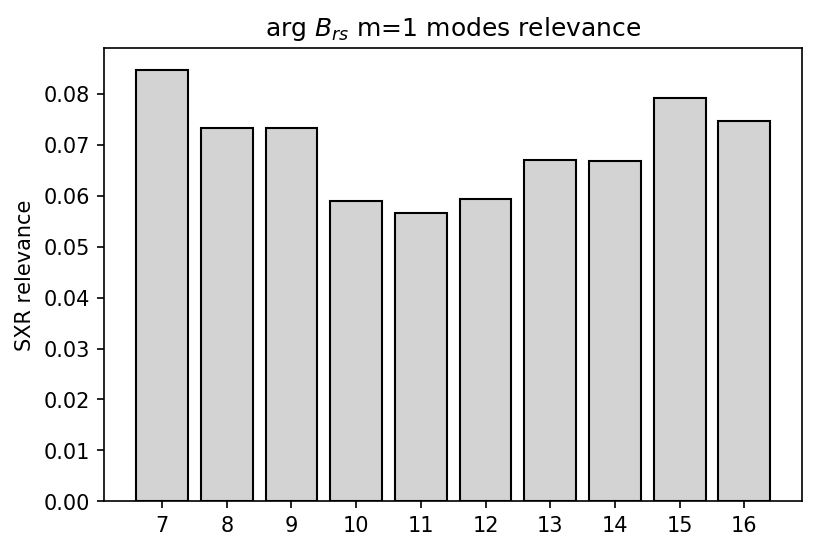
\includegraphics[height=3.3cm]{img/STEP12_7/STEP12_7_arg_Br_rs.png} \label{step_12_7_arg_Brs}}
    \caption{ Training 500 epochs - STEP 12.7 mse, slightly overfitted but validation not diverging }
    \label{fig:step_12_7}
\end{figure}

\begin{figure}
    \centering
    \subfigure{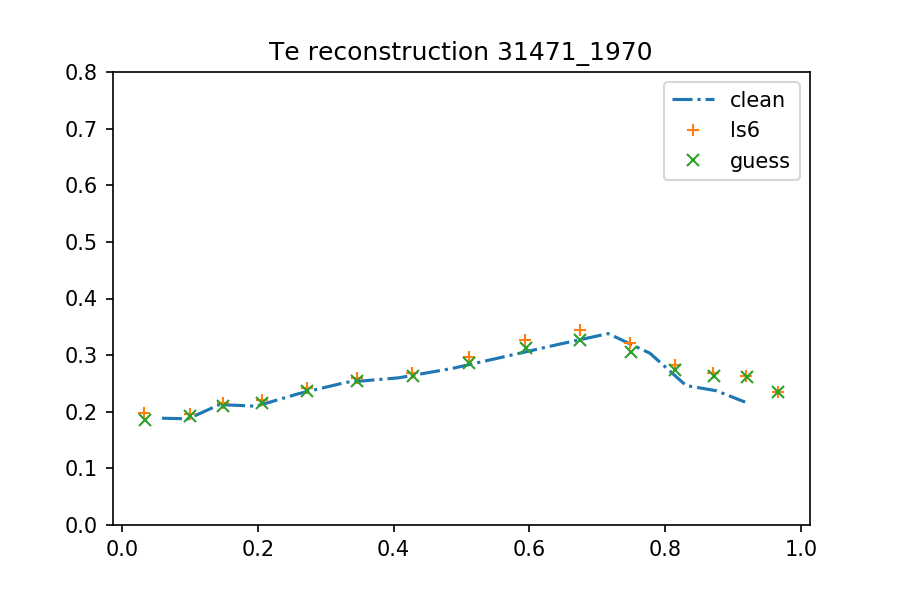
\includegraphics[height=4.8cm]{img/STEP12_7/Te_rec_215.png} }
%   \subfigure{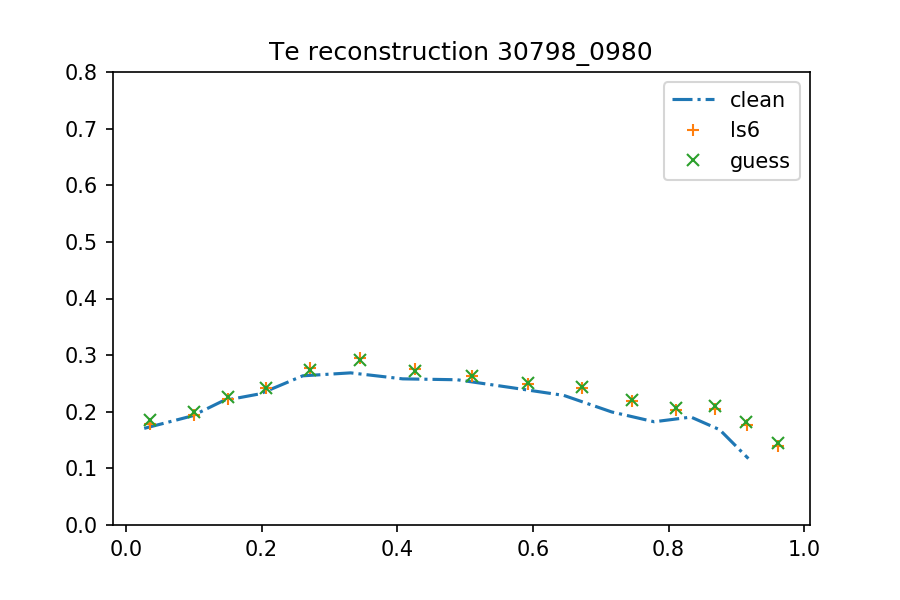
\includegraphics[height=4.8cm]{img/STEP12_7/Te_rec_219.png} }
    \subfigure{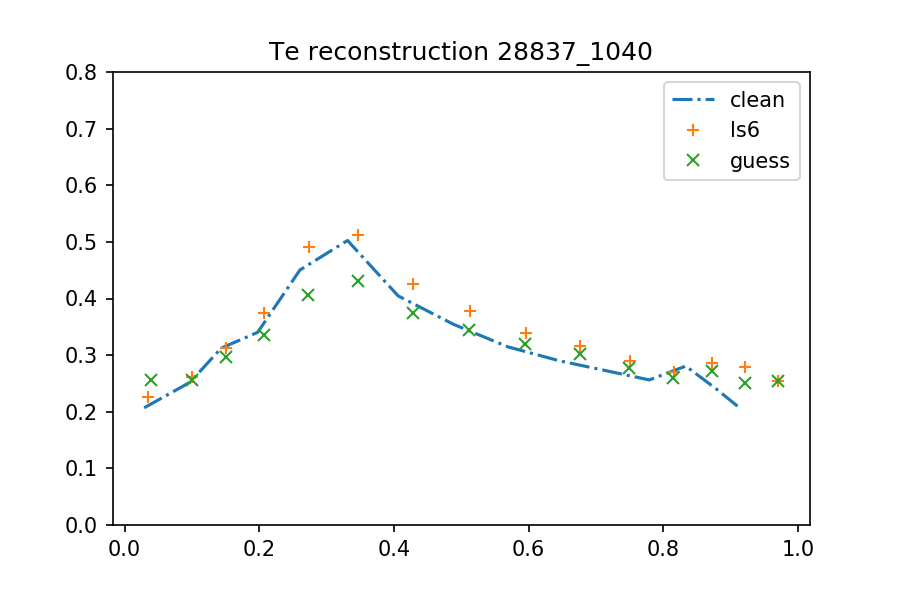
\includegraphics[height=4.8cm]{img/STEP12_7/Te_rec_229.png} }
    \subfigure{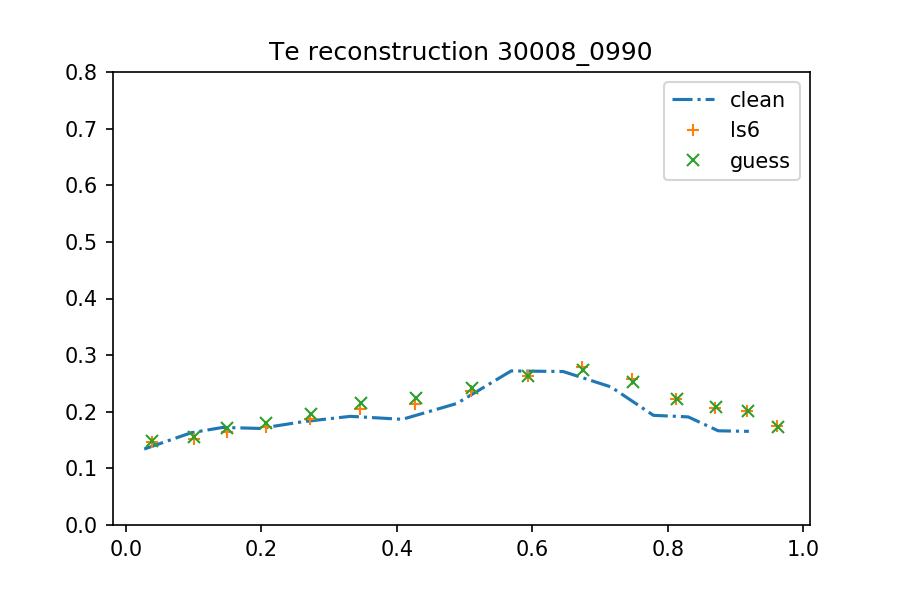
\includegraphics[height=4.8cm]{img/STEP12_7/Te_rec_232.png} }
%   \subfigure{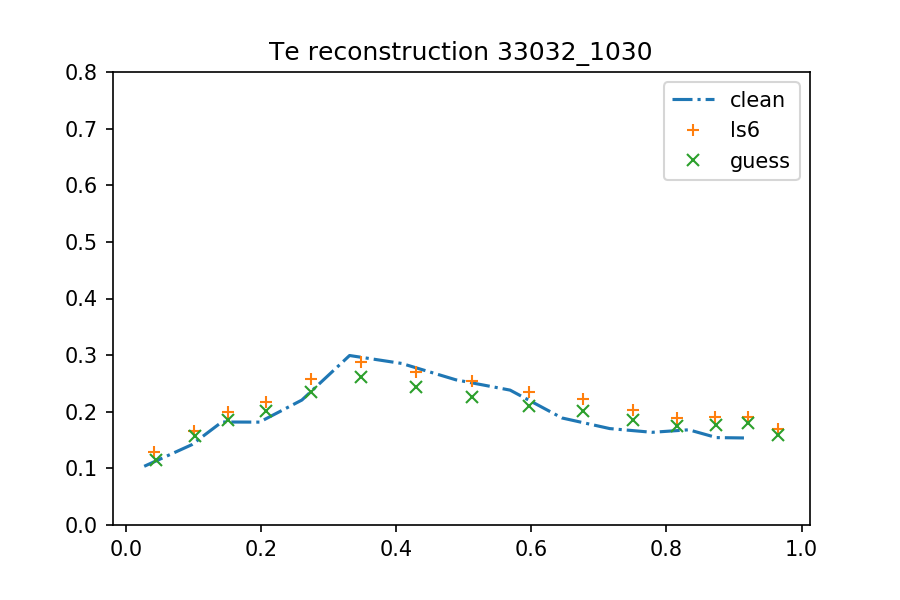
\includegraphics[height=4.8cm]{img/STEP12_7/Te_rec_243.png} }
    \subfigure{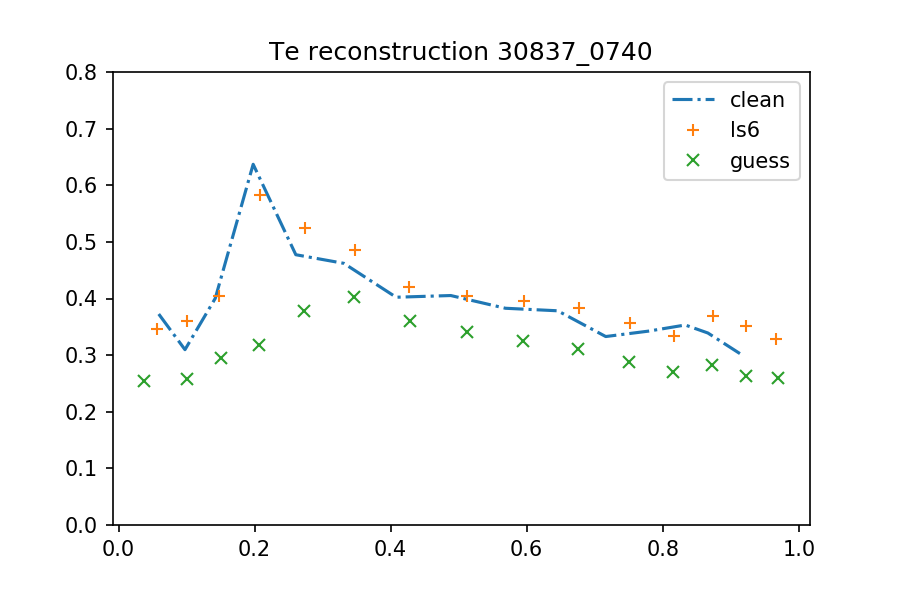
\includegraphics[height=4.8cm]{img/STEP12_7/Te_rec_213.png} }
    \caption{ Training 500 epochs - STEP 12.7 mse, slightly overfitted but validation not diverging }
    \label{fig:step_12_7_rec}
\end{figure}

